\documentclass[1p]{elsarticle_modified}
%\bibliographystyle{elsarticle-num}

%\usepackage[colorlinks]{hyperref}
%\usepackage{abbrmath_seonhwa} %\Abb, \Ascr, \Acal ,\Abf, \Afrak
\usepackage{amsfonts}
\usepackage{amssymb}
\usepackage{amsmath}
\usepackage{amsthm}
\usepackage{scalefnt}
\usepackage{amsbsy}
\usepackage{kotex}
\usepackage{caption}
\usepackage{subfig}
\usepackage{color}
\usepackage{graphicx}
\usepackage{xcolor} %% white, black, red, green, blue, cyan, magenta, yellow
\usepackage{float}
\usepackage{setspace}
\usepackage{hyperref}

\usepackage{tikz}
\usetikzlibrary{arrows}

\usepackage{multirow}
\usepackage{array} % fixed length table
\usepackage{hhline}

%%%%%%%%%%%%%%%%%%%%%
\makeatletter
\renewcommand*\env@matrix[1][\arraystretch]{%
	\edef\arraystretch{#1}%
	\hskip -\arraycolsep
	\let\@ifnextchar\new@ifnextchar
	\array{*\c@MaxMatrixCols c}}
\makeatother %https://tex.stackexchange.com/questions/14071/how-can-i-increase-the-line-spacing-in-a-matrix
%%%%%%%%%%%%%%%

\usepackage[normalem]{ulem}

\newcommand{\msout}[1]{\ifmmode\text{\sout{\ensuremath{#1}}}\else\sout{#1}\fi}
%SOURCE: \msout is \stkout macro in https://tex.stackexchange.com/questions/20609/strikeout-in-math-mode

\newcommand{\cancel}[1]{
	\ifmmode
	{\color{red}\msout{#1}}
	\else
	{\color{red}\sout{#1}}
	\fi
}

\newcommand{\add}[1]{
	{\color{blue}\uwave{#1}}
}

\newcommand{\replace}[2]{
	\ifmmode
	{\color{red}\msout{#1}}{\color{blue}\uwave{#2}}
	\else
	{\color{red}\sout{#1}}{\color{blue}\uwave{#2}}
	\fi
}

\newcommand{\Sol}{\mathcal{S}} %segment
\newcommand{\D}{D} %diagram
\newcommand{\A}{\mathcal{A}} %arc


%%%%%%%%%%%%%%%%%%%%%%%%%%%%%5 test

\def\sl{\operatorname{\textup{SL}}(2,\Cbb)}
\def\psl{\operatorname{\textup{PSL}}(2,\Cbb)}
\def\quan{\mkern 1mu \triangleright \mkern 1mu}

\theoremstyle{definition}
\newtheorem{thm}{Theorem}[section]
\newtheorem{prop}[thm]{Proposition}
\newtheorem{lem}[thm]{Lemma}
\newtheorem{ques}[thm]{Question}
\newtheorem{cor}[thm]{Corollary}
\newtheorem{defn}[thm]{Definition}
\newtheorem{exam}[thm]{Example}
\newtheorem{rmk}[thm]{Remark}
\newtheorem{alg}[thm]{Algorithm}

\newcommand{\I}{\sqrt{-1}}
\begin{document}

%\begin{frontmatter}
%
%\title{Boundary parabolic representations of knots up to 8 crossings}
%
%%% Group authors per affiliation:
%\author{Yunhi Cho} 
%\address{Department of Mathematics, University of Seoul, Seoul, Korea}
%\ead{yhcho@uos.ac.kr}
%
%
%\author{Seonhwa Kim} %\fnref{s_kim}}
%\address{Center for Geometry and Physics, Institute for Basic Science, Pohang, 37673, Korea}
%\ead{ryeona17@ibs.re.kr}
%
%\author{Hyuk Kim}
%\address{Department of Mathematical Sciences, Seoul National University, Seoul 08826, Korea}
%\ead{hyukkim@snu.ac.kr}
%
%\author{Seokbeom Yoon}
%\address{Department of Mathematical Sciences, Seoul National University, Seoul, 08826,  Korea}
%\ead{sbyoon15@snu.ac.kr}
%
%\begin{abstract}
%We find all boundary parabolic representation of knots up to 8 crossings.
%
%\end{abstract}
%\begin{keyword}
%    \MSC[2010] 57M25 
%\end{keyword}
%
%\end{frontmatter}

%\linenumbers
%\tableofcontents
%
\newcommand\colored[1]{\textcolor{white}{\rule[-0.35ex]{0.8em}{1.4ex}}\kern-0.8em\color{red} #1}%
%\newcommand\colored[1]{\textcolor{white}{ #1}\kern-2.17ex	\textcolor{white}{ #1}\kern-1.81ex	\textcolor{white}{ #1}\kern-2.15ex\color{red}#1	}

{\Large $\underline{11a_{159}~(K11a_{159})}$}

\setlength{\tabcolsep}{10pt}
\renewcommand{\arraystretch}{1.6}
\vspace{1cm}\begin{tabular}{m{100pt}>{\centering\arraybackslash}m{274pt}}
\multirow{5}{120pt}{
	\centering
	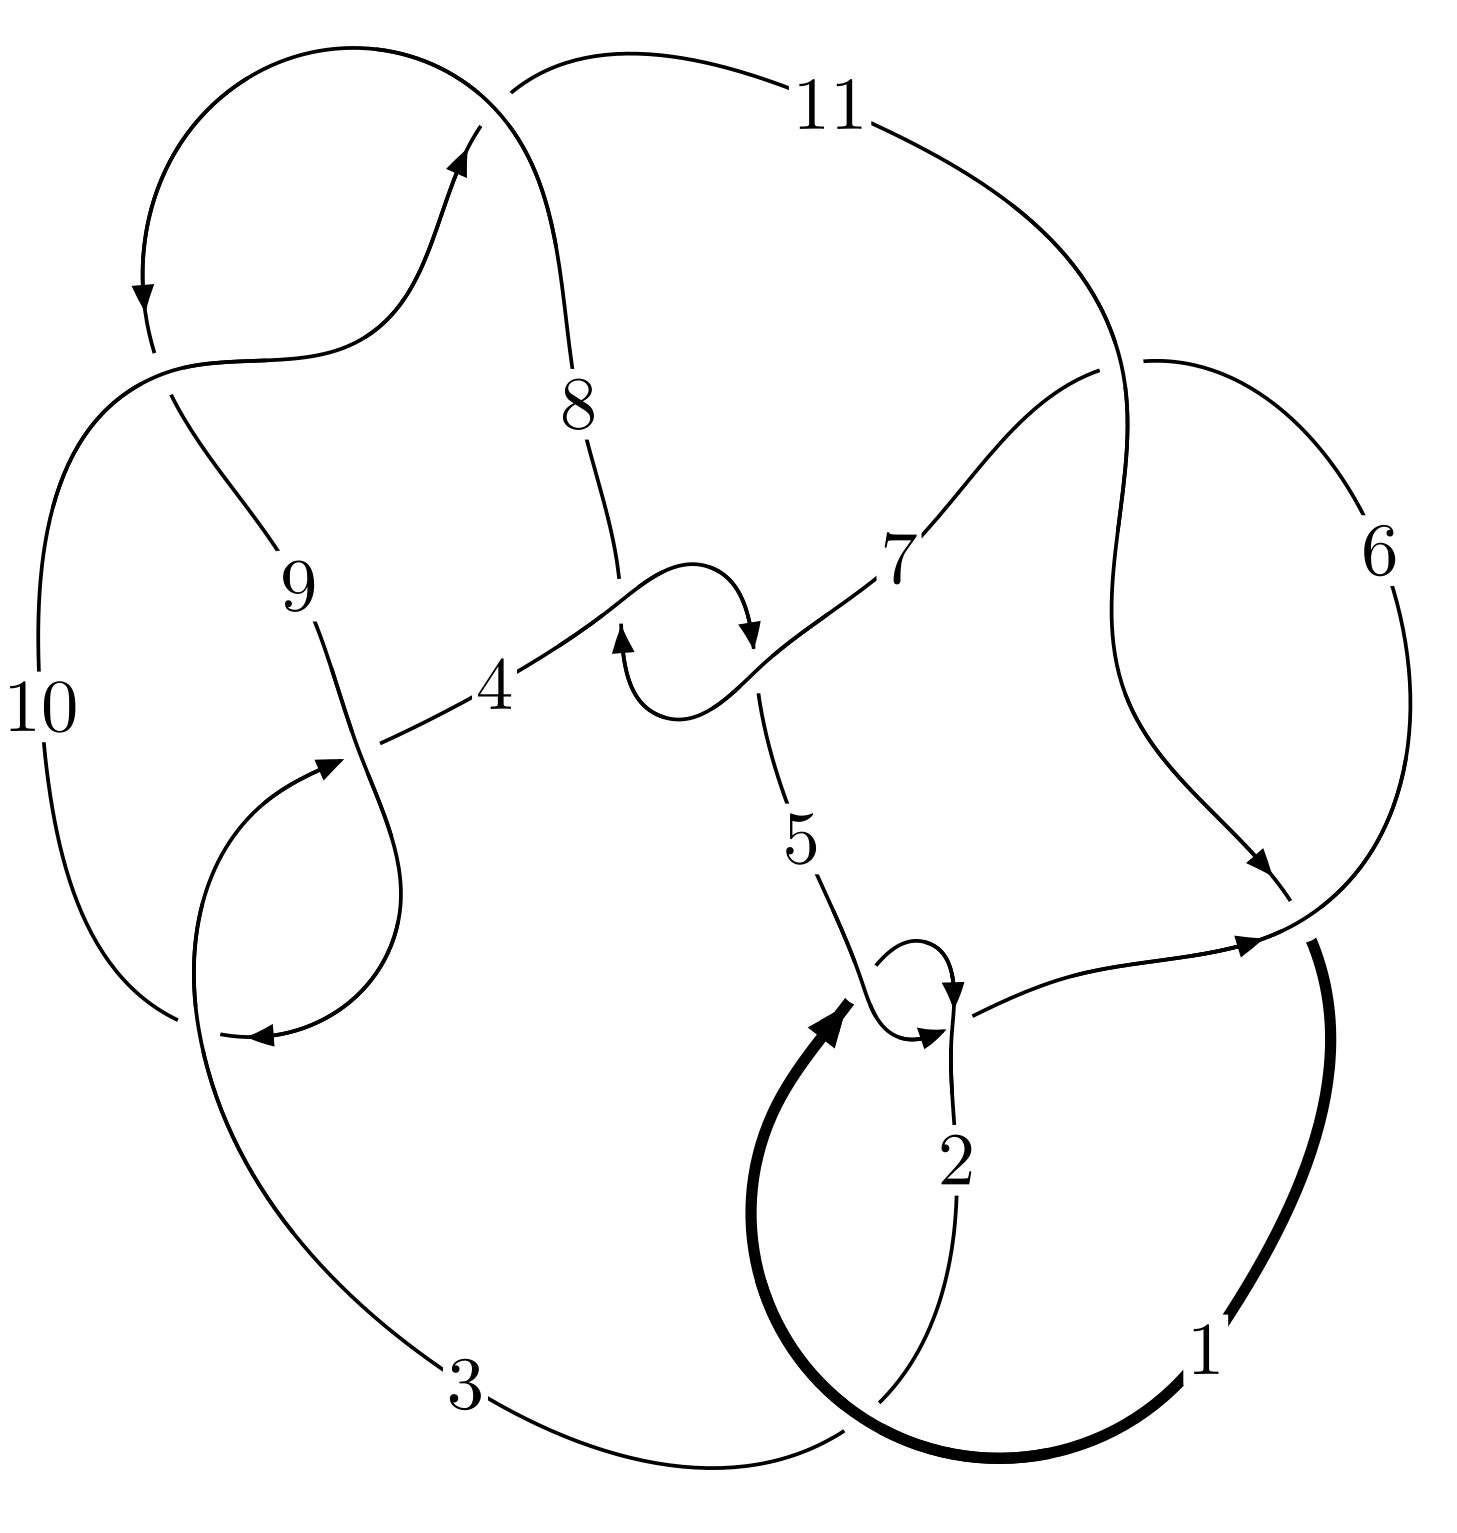
\includegraphics[width=112pt]{../../../GIT/diagram.site/Diagrams/png/408_11a_159.png}\\
\ \ \ A knot diagram\footnotemark}&
\allowdisplaybreaks
\textbf{Linearized knot diagam} \\
\cline{2-2}
 &
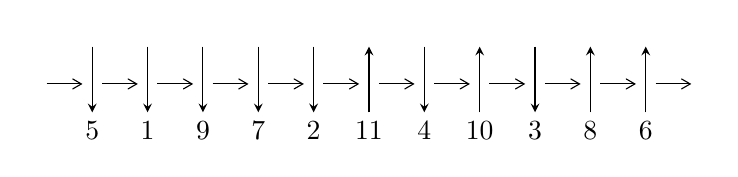
\begin{tikzpicture}[x=20pt, y=17pt]
	% nodes
	\node (C0) at (0, 0) {};
	\node (C1) at (1, 0) {};
	\node (C1U) at (1, +1) {};
	\node (C1D) at (1, -1) {5};

	\node (C2) at (2, 0) {};
	\node (C2U) at (2, +1) {};
	\node (C2D) at (2, -1) {1};

	\node (C3) at (3, 0) {};
	\node (C3U) at (3, +1) {};
	\node (C3D) at (3, -1) {9};

	\node (C4) at (4, 0) {};
	\node (C4U) at (4, +1) {};
	\node (C4D) at (4, -1) {7};

	\node (C5) at (5, 0) {};
	\node (C5U) at (5, +1) {};
	\node (C5D) at (5, -1) {2};

	\node (C6) at (6, 0) {};
	\node (C6U) at (6, +1) {};
	\node (C6D) at (6, -1) {11};

	\node (C7) at (7, 0) {};
	\node (C7U) at (7, +1) {};
	\node (C7D) at (7, -1) {4};

	\node (C8) at (8, 0) {};
	\node (C8U) at (8, +1) {};
	\node (C8D) at (8, -1) {10};

	\node (C9) at (9, 0) {};
	\node (C9U) at (9, +1) {};
	\node (C9D) at (9, -1) {3};

	\node (C10) at (10, 0) {};
	\node (C10U) at (10, +1) {};
	\node (C10D) at (10, -1) {8};

	\node (C11) at (11, 0) {};
	\node (C11U) at (11, +1) {};
	\node (C11D) at (11, -1) {6};
	\node (C12) at (12, 0) {};

	% arrows
	\draw[->,>={angle 60}]
	(C0) edge (C1) (C1) edge (C2) (C2) edge (C3) (C3) edge (C4) (C4) edge (C5) (C5) edge (C6) (C6) edge (C7) (C7) edge (C8) (C8) edge (C9) (C9) edge (C10) (C10) edge (C11) (C11) edge (C12) ;	\draw[->,>=stealth]
	(C1U) edge (C1D) (C2U) edge (C2D) (C3U) edge (C3D) (C4U) edge (C4D) (C5U) edge (C5D) (C6D) edge (C6U) (C7U) edge (C7D) (C8D) edge (C8U) (C9U) edge (C9D) (C10D) edge (C10U) (C11D) edge (C11U) ;
	\end{tikzpicture} \\
\hhline{~~} \\& 
\textbf{Solving Sequence} \\ \cline{2-2} 
 &
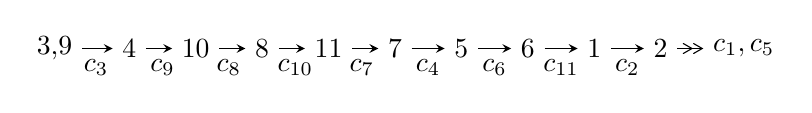
\begin{tikzpicture}[x=24pt, y=7pt]
	% node
	\node (A0) at (-1/8, 0) {3,9};
	\node (A1) at (1, 0) {4};
	\node (A2) at (2, 0) {10};
	\node (A3) at (3, 0) {8};
	\node (A4) at (4, 0) {11};
	\node (A5) at (5, 0) {7};
	\node (A6) at (6, 0) {5};
	\node (A7) at (7, 0) {6};
	\node (A8) at (8, 0) {1};
	\node (A9) at (9, 0) {2};
	\node (C1) at (1/2, -1) {$c_{3}$};
	\node (C2) at (3/2, -1) {$c_{9}$};
	\node (C3) at (5/2, -1) {$c_{8}$};
	\node (C4) at (7/2, -1) {$c_{10}$};
	\node (C5) at (9/2, -1) {$c_{7}$};
	\node (C6) at (11/2, -1) {$c_{4}$};
	\node (C7) at (13/2, -1) {$c_{6}$};
	\node (C8) at (15/2, -1) {$c_{11}$};
	\node (C9) at (17/2, -1) {$c_{2}$};
	\node (A10) at (41/4, 0) {$c_{1},c_{5}$};

	% edge
	\draw[->,>=stealth]	
	(A0) edge (A1) (A1) edge (A2) (A2) edge (A3) (A3) edge (A4) (A4) edge (A5) (A5) edge (A6) (A6) edge (A7) (A7) edge (A8) (A8) edge (A9) ;
	\draw[->>,>={angle 60}]	
	(A9) edge (A10);
\end{tikzpicture} \\ 

\end{tabular} \\

\footnotetext{
The image of knot diagram is generated by the software ``\textbf{Draw programme}" developed by Andrew Bartholomew(\url{http://www.layer8.co.uk/maths/draw/index.htm\#Running-draw}), where we modified some parts for our purpose(\url{https://github.com/CATsTAILs/LinksPainter}).
}\phantom \\ \newline 
\centering \textbf{Ideals for irreducible components\footnotemark of $X_{\text{par}}$} 
 
\begin{align*}
I^u_{1}&=\langle 
u^{55}+u^{54}+\cdots+2 u+1\rangle \\
\\
\end{align*}
\raggedright * 1 irreducible components of $\dim_{\mathbb{C}}=0$, with total 55 representations.\\
\footnotetext{All coefficients of polynomials are rational numbers. But the coefficients are sometimes approximated in decimal forms when there is not enough margin.}
\newpage
\renewcommand{\arraystretch}{1}
\centering \section*{I. $I^u_{1}= \langle u^{55}+u^{54}+\cdots+2 u+1 \rangle$}
\flushleft \textbf{(i) Arc colorings}\\
\begin{tabular}{m{7pt} m{180pt} m{7pt} m{180pt} }
\flushright $a_{3}=$&$\begin{pmatrix}1\\0\end{pmatrix}$ \\
\flushright $a_{9}=$&$\begin{pmatrix}0\\u\end{pmatrix}$ \\
\flushright $a_{4}=$&$\begin{pmatrix}1\\u^2\end{pmatrix}$ \\
\flushright $a_{10}=$&$\begin{pmatrix}- u\\u\end{pmatrix}$ \\
\flushright $a_{8}=$&$\begin{pmatrix}- u^3\\u^3+u\end{pmatrix}$ \\
\flushright $a_{11}=$&$\begin{pmatrix}- u^5- u\\u^5+u^3+u\end{pmatrix}$ \\
\flushright $a_{7}=$&$\begin{pmatrix}u^5+u\\u^7+u^5+2 u^3+u\end{pmatrix}$ \\
\flushright $a_{5}=$&$\begin{pmatrix}u^{10}+u^8+2 u^6+u^4+u^2+1\\u^{12}+2 u^{10}+4 u^8+4 u^6+3 u^4+2 u^2\end{pmatrix}$ \\
\flushright $a_{6}=$&$\begin{pmatrix}- u^{17}-2 u^{15}-5 u^{13}-6 u^{11}-7 u^9-6 u^7-2 u^5-2 u^3+u\\u^{17}+3 u^{15}+7 u^{13}+10 u^{11}+11 u^9+10 u^7+6 u^5+4 u^3+u\end{pmatrix}$ \\
\flushright $a_{1}=$&$\begin{pmatrix}- u^{29}-4 u^{27}+\cdots+2 u^3- u\\u^{29}+5 u^{27}+\cdots+3 u^3+u\end{pmatrix}$ \\
\flushright $a_{2}=$&$\begin{pmatrix}- u^{51}-8 u^{49}+\cdots-5 u^3-2 u\\- u^{53}-9 u^{51}+\cdots+u^3+u\end{pmatrix}$\\ \flushright $a_{2}=$&$\begin{pmatrix}- u^{51}-8 u^{49}+\cdots-5 u^3-2 u\\- u^{53}-9 u^{51}+\cdots+u^3+u\end{pmatrix}$\\&\end{tabular}
\flushleft \textbf{(ii) Obstruction class $= -1$}\\~\\
\flushleft \textbf{(iii) Cusp Shapes $= -4 u^{54}-36 u^{52}+\cdots-4 u-6$}\\~\\
\newpage\renewcommand{\arraystretch}{1}
\flushleft \textbf{(iv) u-Polynomials at the component}\newline \\
\begin{tabular}{m{50pt}|m{274pt}}
Crossings & \hspace{64pt}u-Polynomials at each crossing \\
\hline $$\begin{aligned}c_{1},c_{5}\end{aligned}$$&$\begin{aligned}
&u^{55}+u^{54}+\cdots+2 u^3+1
\end{aligned}$\\
\hline $$\begin{aligned}c_{2}\end{aligned}$$&$\begin{aligned}
&u^{55}+29 u^{54}+\cdots-6 u^2+1
\end{aligned}$\\
\hline $$\begin{aligned}c_{3},c_{9}\end{aligned}$$&$\begin{aligned}
&u^{55}+u^{54}+\cdots+2 u+1
\end{aligned}$\\
\hline $$\begin{aligned}c_{4},c_{7}\end{aligned}$$&$\begin{aligned}
&u^{55}-5 u^{54}+\cdots-4 u+1
\end{aligned}$\\
\hline $$\begin{aligned}c_{6},c_{11}\end{aligned}$$&$\begin{aligned}
&u^{55}+3 u^{54}+\cdots+35 u+16
\end{aligned}$\\
\hline $$\begin{aligned}c_{8},c_{10}\end{aligned}$$&$\begin{aligned}
&u^{55}-19 u^{54}+\cdots-18 u^2+1
\end{aligned}$\\
\hline
\end{tabular}\\~\\
\newpage\renewcommand{\arraystretch}{1}
\flushleft \textbf{(v) Riley Polynomials at the component}\newline \\
\begin{tabular}{m{50pt}|m{274pt}}
Crossings & \hspace{64pt}Riley Polynomials at each crossing \\
\hline $$\begin{aligned}c_{1},c_{5}\end{aligned}$$&$\begin{aligned}
&y^{55}-29 y^{54}+\cdots+6 y^2-1
\end{aligned}$\\
\hline $$\begin{aligned}c_{2}\end{aligned}$$&$\begin{aligned}
&y^{55}-5 y^{54}+\cdots+12 y-1
\end{aligned}$\\
\hline $$\begin{aligned}c_{3},c_{9}\end{aligned}$$&$\begin{aligned}
&y^{55}+19 y^{54}+\cdots+18 y^2-1
\end{aligned}$\\
\hline $$\begin{aligned}c_{4},c_{7}\end{aligned}$$&$\begin{aligned}
&y^{55}+31 y^{54}+\cdots-92 y-1
\end{aligned}$\\
\hline $$\begin{aligned}c_{6},c_{11}\end{aligned}$$&$\begin{aligned}
&y^{55}+39 y^{54}+\cdots-6167 y-256
\end{aligned}$\\
\hline $$\begin{aligned}c_{8},c_{10}\end{aligned}$$&$\begin{aligned}
&y^{55}+35 y^{54}+\cdots+36 y-1
\end{aligned}$\\
\hline
\end{tabular}\\~\\
\newpage\flushleft \textbf{(vi) Complex Volumes and Cusp Shapes}
$$\begin{array}{c|c|c}  
\text{Solutions to }I^u_{1}& \I (\text{vol} + \sqrt{-1}CS) & \text{Cusp shape}\\
 \hline 
\begin{aligned}
u &= \phantom{-}0.784082 + 0.635234 I\end{aligned}
 & -1.91993 + 3.95621 I & -4.32723 - 2.21514 I \\ \hline\begin{aligned}
u &= \phantom{-}0.784082 - 0.635234 I\end{aligned}
 & -1.91993 - 3.95621 I & -4.32723 + 2.21514 I \\ \hline\begin{aligned}
u &= -0.799722 + 0.633488 I\end{aligned}
 & -4.89200 - 8.77056 I & -7.47137 + 5.34591 I \\ \hline\begin{aligned}
u &= -0.799722 - 0.633488 I\end{aligned}
 & -4.89200 + 8.77056 I & -7.47137 - 5.34591 I \\ \hline\begin{aligned}
u &= \phantom{-}0.695449 + 0.747109 I\end{aligned}
 & -3.52521 + 0.06578 I & -10.04150 - 0.64430 I \\ \hline\begin{aligned}
u &= \phantom{-}0.695449 - 0.747109 I\end{aligned}
 & -3.52521 - 0.06578 I & -10.04150 + 0.64430 I \\ \hline\begin{aligned}
u &= -0.785485 + 0.659519 I\end{aligned}
 & -5.96663 - 0.17301 I & -9.26357 - 0.91884 I \\ \hline\begin{aligned}
u &= -0.785485 - 0.659519 I\end{aligned}
 & -5.96663 + 0.17301 I & -9.26357 + 0.91884 I \\ \hline\begin{aligned}
u &= \phantom{-}0.515960 + 0.907861 I\end{aligned}
 & -2.45106 - 5.66045 I & -4.09002 + 7.28827 I \\ \hline\begin{aligned}
u &= \phantom{-}0.515960 - 0.907861 I\end{aligned}
 & -2.45106 + 5.66045 I & -4.09002 - 7.28827 I \\ \hline\begin{aligned}
u &= \phantom{-}0.087591 + 1.044510 I\end{aligned}
 & \phantom{-}0.0418156 + 0.0593950 I & -1.97321 + 0.28127 I \\ \hline\begin{aligned}
u &= \phantom{-}0.087591 - 1.044510 I\end{aligned}
 & \phantom{-}0.0418156 - 0.0593950 I & -1.97321 - 0.28127 I \\ \hline\begin{aligned}
u &= \phantom{-}0.732924 + 0.589195 I\end{aligned}
 & \phantom{-}1.02771 + 3.24584 I & -2.27897 - 4.07779 I \\ \hline\begin{aligned}
u &= \phantom{-}0.732924 - 0.589195 I\end{aligned}
 & \phantom{-}1.02771 - 3.24584 I & -2.27897 + 4.07779 I \\ \hline\begin{aligned}
u &= -0.518072 + 0.766150 I\end{aligned}
 & -0.11478 + 1.78039 I & -0.55066 - 3.60054 I \\ \hline\begin{aligned}
u &= -0.518072 - 0.766150 I\end{aligned}
 & -0.11478 - 1.78039 I & -0.55066 + 3.60054 I \\ \hline\begin{aligned}
u &= -0.066273 + 1.075310 I\end{aligned}
 & \phantom{-}4.04900 + 3.40061 I & \phantom{-}3.11315 - 3.08609 I \\ \hline\begin{aligned}
u &= -0.066273 - 1.075310 I\end{aligned}
 & \phantom{-}4.04900 - 3.40061 I & \phantom{-}3.11315 + 3.08609 I \\ \hline\begin{aligned}
u &= -0.013325 + 1.085250 I\end{aligned}
 & \phantom{-}6.52620 + 2.29211 I & \phantom{-}4.76004 - 3.60647 I \\ \hline\begin{aligned}
u &= -0.013325 - 1.085250 I\end{aligned}
 & \phantom{-}6.52620 - 2.29211 I & \phantom{-}4.76004 + 3.60647 I \\ \hline\begin{aligned}
u &= \phantom{-}0.080625 + 1.087480 I\end{aligned}
 & \phantom{-}1.25671 - 8.17694 I & \phantom{-0.000000 -}0. + 6.49947 I \\ \hline\begin{aligned}
u &= \phantom{-}0.080625 - 1.087480 I\end{aligned}
 & \phantom{-}1.25671 + 8.17694 I & \phantom{-0.000000 } 0. - 6.49947 I \\ \hline\begin{aligned}
u &= -0.682148 + 0.562866 I\end{aligned}
 & \phantom{-}1.33027 + 1.15553 I & -1.16546 - 3.23863 I \\ \hline\begin{aligned}
u &= -0.682148 - 0.562866 I\end{aligned}
 & \phantom{-}1.33027 - 1.15553 I & -1.16546 + 3.23863 I \\ \hline\begin{aligned}
u &= \phantom{-}0.741553 + 0.863345 I\end{aligned}
 & -5.44101 - 2.81013 I & -7.05601 + 3.05455 I \\ \hline\begin{aligned}
u &= \phantom{-}0.741553 - 0.863345 I\end{aligned}
 & -5.44101 + 2.81013 I & -7.05601 - 3.05455 I \\ \hline\begin{aligned}
u &= -0.757396 + 0.852445 I\end{aligned}
 & -8.97089 - 1.53080 I & -10.56468 + 0. I\phantom{ +0.000000I} \\ \hline\begin{aligned}
u &= -0.757396 - 0.852445 I\end{aligned}
 & -8.97089 + 1.53080 I & -10.56468 + 0. I\phantom{ +0.000000I} \\ \hline\begin{aligned}
u &= \phantom{-}0.578305 + 0.998594 I\end{aligned}
 & -1.71452 + 1.81047 I & \phantom{-0.000000 } 0 \\ \hline\begin{aligned}
u &= \phantom{-}0.578305 - 0.998594 I\end{aligned}
 & -1.71452 - 1.81047 I & \phantom{-0.000000 } 0\\
 \hline 
 \end{array}$$\newpage$$\begin{array}{c|c|c}  
\text{Solutions to }I^u_{1}& \I (\text{vol} + \sqrt{-1}CS) & \text{Cusp shape}\\
 \hline 
\begin{aligned}
u &= \phantom{-}0.663907 + 0.946346 I\end{aligned}
 & -2.91576 - 5.31435 I & -7.80390 + 6.55381 I \\ \hline\begin{aligned}
u &= \phantom{-}0.663907 - 0.946346 I\end{aligned}
 & -2.91576 + 5.31435 I & -7.80390 - 6.55381 I \\ \hline\begin{aligned}
u &= -0.751586 + 0.878593 I\end{aligned}
 & -8.89140 + 7.22930 I & -10.25643 - 6.47034 I \\ \hline\begin{aligned}
u &= -0.751586 - 0.878593 I\end{aligned}
 & -8.89140 - 7.22930 I & -10.25643 + 6.47034 I \\ \hline\begin{aligned}
u &= -0.606564 + 0.990704 I\end{aligned}
 & \phantom{-}0.84076 + 2.75512 I & \phantom{-0.000000 } 0 \\ \hline\begin{aligned}
u &= -0.606564 - 0.990704 I\end{aligned}
 & \phantom{-}0.84076 - 2.75512 I & \phantom{-0.000000 } 0 \\ \hline\begin{aligned}
u &= -0.644080 + 1.018780 I\end{aligned}
 & \phantom{-}2.61827 + 4.00138 I & \phantom{-0.000000 } 0 \\ \hline\begin{aligned}
u &= -0.644080 - 1.018780 I\end{aligned}
 & \phantom{-}2.61827 - 4.00138 I & \phantom{-0.000000 } 0 \\ \hline\begin{aligned}
u &= \phantom{-}0.660956 + 1.025220 I\end{aligned}
 & \phantom{-}2.29946 - 8.58321 I & \phantom{-0.000000 } 0 \\ \hline\begin{aligned}
u &= \phantom{-}0.660956 - 1.025220 I\end{aligned}
 & \phantom{-}2.29946 + 8.58321 I & \phantom{-0.000000 } 0 \\ \hline\begin{aligned}
u &= -0.698488 + 1.015790 I\end{aligned}
 & -4.89384 + 5.78358 I & \phantom{-0.000000 } 0 \\ \hline\begin{aligned}
u &= -0.698488 - 1.015790 I\end{aligned}
 & -4.89384 - 5.78358 I & \phantom{-0.000000 } 0 \\ \hline\begin{aligned}
u &= \phantom{-}0.690811 + 1.025790 I\end{aligned}
 & -0.74984 - 9.53517 I & \phantom{-0.000000 } 0 \\ \hline\begin{aligned}
u &= \phantom{-}0.690811 - 1.025790 I\end{aligned}
 & -0.74984 + 9.53517 I & \phantom{-0.000000 } 0 \\ \hline\begin{aligned}
u &= -0.696320 + 1.031360 I\end{aligned}
 & -3.6961 + 14.4089 I & \phantom{-0.000000 } 0 \\ \hline\begin{aligned}
u &= -0.696320 - 1.031360 I\end{aligned}
 & -3.6961 - 14.4089 I & \phantom{-0.000000 } 0 \\ \hline\begin{aligned}
u &= -0.171816 + 0.720092 I\end{aligned}
 & \phantom{-}0.95831 + 1.60933 I & \phantom{-}1.49417 - 5.74918 I \\ \hline\begin{aligned}
u &= -0.171816 - 0.720092 I\end{aligned}
 & \phantom{-}0.95831 - 1.60933 I & \phantom{-}1.49417 + 5.74918 I \\ \hline\begin{aligned}
u &= \phantom{-}0.630067 + 0.344372 I\end{aligned}
 & -3.34533 - 6.30811 I & -7.15638 + 6.23846 I \\ \hline\begin{aligned}
u &= \phantom{-}0.630067 - 0.344372 I\end{aligned}
 & -3.34533 + 6.30811 I & -7.15638 - 6.23846 I \\ \hline\begin{aligned}
u &= -0.561648 + 0.367518 I\end{aligned}
 & -0.48181 + 1.78744 I & -3.72385 - 3.38377 I \\ \hline\begin{aligned}
u &= -0.561648 - 0.367518 I\end{aligned}
 & -0.48181 - 1.78744 I & -3.72385 + 3.38377 I \\ \hline\begin{aligned}
u &= \phantom{-}0.569392 + 0.257173 I\end{aligned}
 & -4.05721 + 1.86906 I & -9.08122 - 0.59288 I \\ \hline\begin{aligned}
u &= \phantom{-}0.569392 - 0.257173 I\end{aligned}
 & -4.05721 - 1.86906 I & -9.08122 + 0.59288 I \\ \hline\begin{aligned}
u &= -0.357397\phantom{ +0.000000I}\end{aligned}
 & -1.02390\phantom{ +0.000000I} & -10.8300\phantom{ +0.000000I}\\
 \hline 
 \end{array}$$\newpage
\newpage\renewcommand{\arraystretch}{1}
\centering \section*{ II. u-Polynomials}
\begin{tabular}{m{50pt}|m{274pt}}
Crossings & \hspace{64pt}u-Polynomials at each crossing \\
\hline $$\begin{aligned}c_{1},c_{5}\end{aligned}$$&$\begin{aligned}
&u^{55}+u^{54}+\cdots+2 u^3+1
\end{aligned}$\\
\hline $$\begin{aligned}c_{2}\end{aligned}$$&$\begin{aligned}
&u^{55}+29 u^{54}+\cdots-6 u^2+1
\end{aligned}$\\
\hline $$\begin{aligned}c_{3},c_{9}\end{aligned}$$&$\begin{aligned}
&u^{55}+u^{54}+\cdots+2 u+1
\end{aligned}$\\
\hline $$\begin{aligned}c_{4},c_{7}\end{aligned}$$&$\begin{aligned}
&u^{55}-5 u^{54}+\cdots-4 u+1
\end{aligned}$\\
\hline $$\begin{aligned}c_{6},c_{11}\end{aligned}$$&$\begin{aligned}
&u^{55}+3 u^{54}+\cdots+35 u+16
\end{aligned}$\\
\hline $$\begin{aligned}c_{8},c_{10}\end{aligned}$$&$\begin{aligned}
&u^{55}-19 u^{54}+\cdots-18 u^2+1
\end{aligned}$\\
\hline
\end{tabular}\newpage\renewcommand{\arraystretch}{1}
\centering \section*{ III. Riley Polynomials}
\begin{tabular}{m{50pt}|m{274pt}}
Crossings & \hspace{64pt}Riley Polynomials at each crossing \\
\hline $$\begin{aligned}c_{1},c_{5}\end{aligned}$$&$\begin{aligned}
&y^{55}-29 y^{54}+\cdots+6 y^2-1
\end{aligned}$\\
\hline $$\begin{aligned}c_{2}\end{aligned}$$&$\begin{aligned}
&y^{55}-5 y^{54}+\cdots+12 y-1
\end{aligned}$\\
\hline $$\begin{aligned}c_{3},c_{9}\end{aligned}$$&$\begin{aligned}
&y^{55}+19 y^{54}+\cdots+18 y^2-1
\end{aligned}$\\
\hline $$\begin{aligned}c_{4},c_{7}\end{aligned}$$&$\begin{aligned}
&y^{55}+31 y^{54}+\cdots-92 y-1
\end{aligned}$\\
\hline $$\begin{aligned}c_{6},c_{11}\end{aligned}$$&$\begin{aligned}
&y^{55}+39 y^{54}+\cdots-6167 y-256
\end{aligned}$\\
\hline $$\begin{aligned}c_{8},c_{10}\end{aligned}$$&$\begin{aligned}
&y^{55}+35 y^{54}+\cdots+36 y-1
\end{aligned}$\\
\hline
\end{tabular}
\vskip 2pc
\end{document}